\scanpage{109}
% archive foliation: 108
\[
\begin{aligned}
\lambda(P(c)u+Q(c))&=1\\
\lambda(P(c)v+Q(c))&=1
\end{aligned}
\]
\[P(c)(u-v)=0\]
\[\boxed{P(c)=0}\qquad\lambda=\frac1{Q(c)}\]
\[Q(c)\ne0\]
\figure{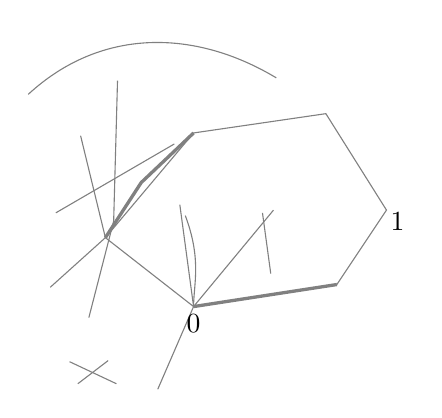
\begin{tikzpicture}[scale=.7]
\draw[gray](-2,2.8)..controls(-.7,4)and(1,4)..(2.5,3.1);
\draw[gray](-.6,.2)--(1,2.1)--(3.4,2.45)--(4.5,.7)--(3.6,-.65)--(1,-1.05)--cycle;
\draw[gray,line width=1.2pt](-.6,.2)--(.05,1.2)--(1,2.1);\draw[gray,line width=1.2pt](1,-1.05)--(3.6,-.65);
\draw[gray](-1.6,-.7)--(-.6,.2)--(-1.05,2.05);\draw[gray](-.9,-1.25)--(-.45,.5)--(-.38,3.05);\draw[gray](-1.5,.65)--(.65,1.9);
\draw[gray](.35,-2.55)--(1,-1.05)--(.75,.8);\draw[gray](.85,.6)..controls(1.15,-.2)and(1,-.65)..(1,-1.05);\draw[gray](1,-1.05)--(2.45,.7);\draw[gray](2.4,-.45)--(2.25,.65);
\draw[gray](-1.25,-2.05)--(-.4,-2.45);\draw[gray](-1.1,-2.45)--(-.55,-2.03);
\node at(1,-1.35){$0$};\node at(4.7,.5){$1$};\end{tikzpicture}}
\margin{$\unsure{\widetilde X}\quad\underline a$}

\[\unsure{\mathcal P}\qquad
\boxed{\begin{array}{l}c\ne0,1\\Q(c)\ne0\\P(c)=0\end{array}}\qquad
f(z)=\frac1{Q(c)}z^3(z-1)^2(z-c)
\]
\[\boxed{(5c+4)^2-72c\ne0}\]
\figure{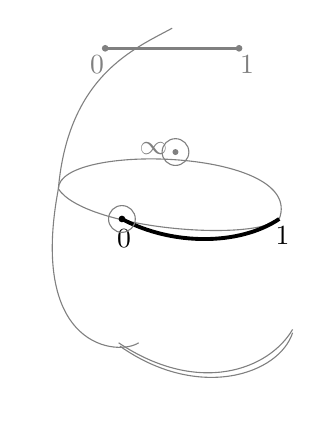
\begin{tikzpicture}[scale=.85]
\draw[gray,line width=1.2pt](0,2.5)--(2,2.5);\fill[gray](0,2.5)circle(.05);\fill[gray](2,2.5)circle(.05);\node[gray]at(-.12,2.25){$0$};\node[gray]at(2.12,2.25){$1$};
\draw[gray](-.7,.4)..controls(-.55,2.1)and(.45,2.5)..(1,2.8);\draw[gray](-.7,.4)..controls(-1.15,-2)and(.2,-2.1)..(.5,-1.9);\draw[gray](-.7,.4)..controls(-.3,-.2)and(2.2,-.4)..(2.6,-.05)..controls(3,1)and(-.7,1.1)..(-.7,.4);
\draw[gray](.2,-1.9)..controls(1.4,-2.7)and(2.45,-2.3)..(2.8,-1.7);\draw[gray](.22,-1.95)..controls(1.4,-2.78)and(2.6,-2.37)..(2.8,-1.75);
\draw[line width=1.4pt](.25,-.05)..controls(1,-.45)and(2,-.45)..(2.6,-.05);\fill(.25,-.05)circle(.05);\node at(.28,-.35){$0$};\node at(2.65,-.3){$1$};\draw[gray](.25,-.05)circle(.2);
\fill[gray](1.05,.95)circle(.045);\draw[gray](1.05,.95)circle(.2);\node[gray]at(.72,1){$\infty$};\end{tikzpicture}}
\figure{
\begin{tikzpicture}[scale=.6]\draw[gray](-.7,-.6)--(.7,.6);\draw[gray](-.65,-.62)--(.75,.58);\draw[gray](-.65,.65)--(.65,-.65);\draw[gray](-.6,.68)--(.72,-.63);\draw[gray](-.82,-.65)--(-.58,-.58);\draw[gray](.58,-.72)--(.82,-.64);\end{tikzpicture}}

$u,v$ sont les racines de
\[\deleted{\unsure{f(z)}}\ z^2-\frac{5c+4}{6}z+\frac c2=0\]
$x,y$ sont les racines de
\figure{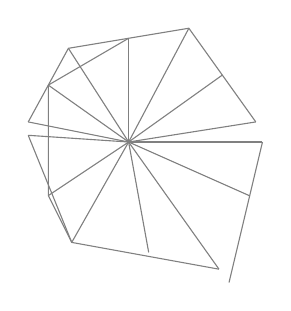
\begin{tikzpicture}[scale=.85]
\coordinate(O)at(0,0);\draw[gray](-1.5,.3)--(-.9,1.4)--(.9,1.7)--(1.9,.3);\draw[gray](-1.5,.1)--(-.85,-1.5)--(1.35,-1.9);\draw[gray](2,0)--(1.5,-2.1);
\foreach\p in{(-1.5,.3),(-1.2,.85),(-.9,1.4),(0,1.55),(.9,1.7),(1.4,1),(1.9,.3),(2,0),(1.8,-.8),(1.35,-1.9),(.3,-1.65),(-.85,-1.5),(-1.2,-.8),(-1.5,.1)}{\draw[gray](O)--\p;}
\draw[gray](-1.2,.85)--(-1.2,-.8)--(-.85,-1.5);\draw[gray](-1.2,.85)--(0,1.55);\end{tikzpicture}}
\[
\frac{f(z)-1}{(z-u)^2(z-v)^2}=\frac{f(z)\unsure{+|-}1}{\left(z^2-\frac{5c+4}{6}z+\frac c2\right)^2}
\]
